\documentclass[12pt]{article}
\usepackage[a4paper, margin=.30in]{geometry}
\usepackage{graphicx ,
            wrapfig,
            xcolor, 
            enumerate,
            amsmath,fontenc,
            tcolorbox,mathrsfs
            }
\usepackage{mathptmx}
\usepackage[siunitx, RPvoltages]{circuitikz}
\newcommand\headerMe[2]{\noindent{}#1\hfill#2}
\renewcommand{\thesection}{\Roman{section}}

\author{Zakaria HAOUZAN}
\date{\today}

\begin{document}
% headers --------------
\headerMe{Matière : Physique-Chimie}{Professeur : Zakaria HAOUZAN}\\
\headerMe{Unité : Electricité}{Établissement : Lycée SKHOR qualifiant}\\
\headerMe{Niveau : 1BAC-SM/X}{Heure : 12H/6H}\\

% ------Content ________

%\begin{wrapfigure}[10]{r}{0.5\textwidth}
    %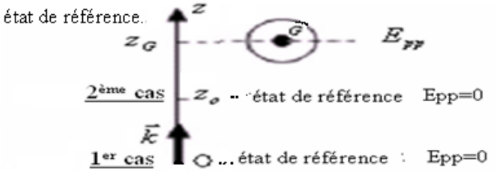
\includegraphics[width=0.5\textwidth]{./img/img00.png}
%\end{wrapfigure}


%\begin{tcolorbox}[colback=black!15!white,
                  %colframe=black!10!black,
                  %title=Remarque :
                 %]
\begin{center}

    \Large{Leçon $N^{\circ} 8 $: \color{red}Comportement global d’un circuit }
\end{center}

\begin{wrapfigure}[10]{r}{0.4\textwidth}
  \vspace{-1cm}
    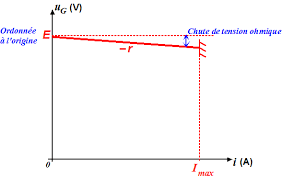
\includegraphics[width=0.4\textwidth]{./img/img_00.png}
\end{wrapfigure}
  \section{Distribution de l’énergie électrique au niveau d’un générateur :}
\subsection{Caractéristique d’un générateur : }
  La caractéristique d’un générateur est la représentation graphique $U_{PN} = f(I)$, c’est une fonction linéaire décroissante.

  La tension électrique UPN aux bornes d’un générateur est : $U_{PN} = E-rI$
  
  E : force électromotrice en (V)

  r : la résistance interne en $(\Omega)$

I : Intensité du courant en(A)

  Symbole d'un générateur dans un circuit électrique : 
  \begin{circuitikz}[european]
    \draw (0,0) to[battery1,v=U,i=I] (2,0);
    
  \end{circuitikz}
\subsection{Bilan énergétique d’un générateur :}
  La tension électrique $U_{PN}$ aux bornes d’un générateur s’écrit : 
  $U_{PN} = E - rI$
  On multipliant les deux membres de cette égalité par I. $\Delta{t}$, on obtient :

  $$U_{PN}.I. \Delta{t} = E. I. \Delta{t} - r. I. \Delta{t}$$
  $$ E. I. \Delta{t}= U_{PN}.I. \Delta{t} + r. I. \Delta{t}$$
  $$W_T = W_U + W_J $$
Tel que  :
  
  $W_T = E. I. \Delta{t}$ : Energie électrique totale fournie par le générateur.

  $W_U = E. I. \Delta{t}$ : Energie électrique utile fournie par le générateur au reste du circuit.

  $W_J = r. I^2.\Delta{t}$ : Energie thermique dissipée par effet Joule dans le générateur.

Donc une partie de l’énergie totale fournie par le générateur est dissipée par effet Joule au niveau sa résistance interne et l’autre
partie est reçue par le circuit .

  On sait $P = \frac{W}{\Delta{t}}$
  donc 
  On divisant les deux membres de l’égalité par $\Delta{t}$, on obtient :

  $P_T = E. I$ : Puissance électrique totale fournie par le générateur au reste du circuit.

  $P_U = U_{PN}. I$ : Puissance électrique utile fournie par le générateur au reste du circuit.

  $P_J = r.I$: Puissance thermique dissipée par effet Joule dans le générateur.

  \subsection{Rendement d’un générateur :}
  Le rendement d’un générateur est le rapport de la puissance utile sur la puissance totale fournie par le générateur .
  $$\rho = \frac{P_U}{P_T} = \frac{U_{PN}.I}{E.I}$$
  $$ \frac{U_{PN}}{E} = \frac{E-r.I}{E} = 1-\frac{rI}{E}$$

$\rho < 1 $ le rendement est une grandeur sans unité Elle est souvent en pourcentage.

Exemple : pour $E = 6V$ On a $r = 1\Omega$ donc $$\rho = 1 - \frac{rI}{E} = 94\%$$
-Plus que la résistance interne du générateur est petite plus que son rendement est grand.


\begin{wrapfigure}[10]{r}{0.4\textwidth}
  \vspace{-1cm}
    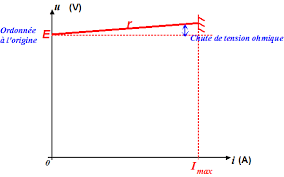
\includegraphics[width=0.4\textwidth]{./img/img_U_r.png}
\end{wrapfigure}

\section{Distribution de l’énergie électrique au niveau d’un récepteur :}
Le récepteur électrique est un dipole qui reçoit l’énergie électrique et la transforme en une autre forme d’énergie.
La caractéristique d’un récepteur est la représentation graphique UPN = f(I), c’ est une fonction linéaire croissante.

  L'expression de la tension aux bornes du récepteur : $$U_{AB} = E' + r'I$$ 
  E' : force électromotrice du générateur (V)

  r' : la résistance interne en $(\Omega)$

  I : Intensité du courant en(A)

En convention $U_{AB}$ et I sont de sens contraires

la courbe qui représente $U_{AB}$ en fonction de I est une droite, son coefficient directeur est égale r' = $\frac{\Delta{U_{AB}}}{\Delta{I}}$

Cas du conducteur ohmique : c’est un cas particulier la tension entre ses bornes est donnée par la loi d’ohm : U=R.I , Il transforme toute l'énergie électrique qu'il reçoit en énergie thermique.

\begin{center}
  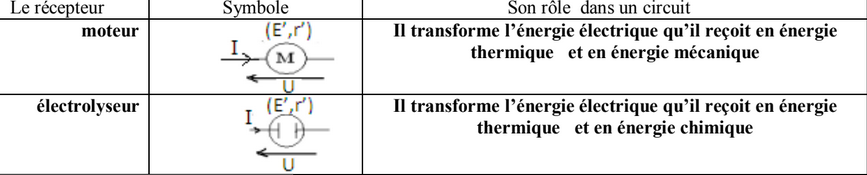
\includegraphics[width=0.7\textwidth]{./img/Exemples _recepteur.png}
\end{center}

\subsection{Bilan énergétique d’un récepteur :}
Expression de la tension aux bornes du récepteur : $U_{AB}=E’+r’.I$

En multipliant les deux membres de cette égalité par $I.\Delta{t}$  :  $U_{AB}.I. \Delta{t} = E'. I. \Delta{t} + r'. I^2. \Delta{t}$
  $$W_e = W_u + W_J $$
Tel que  :  
  $W_e = U_{AB}. I. \Delta{t}$ :est l’énergie électrique reçue par le récepteur. 

  $W_u = E'. I. \Delta{t}$ : est l’énergie utile (qui peut être chimique ou mécanique).

  $W_J = r'. I^2.\Delta{t}$ : Energie thermique dissipée par effet Joule dans le générateur.

Donc une partie de l’énergie totale reçue par le récepteur est dissipée par effet Joule au niveau de sa résistance interne et l’autre
partie est transformée en une autre forme d’énergie (qui est utile).

$P_e = U_{AB}.I$ : est la puissance électrique reçue par le récepteur.

$P_u= E'.I$ : est la puissance utile (qui peut être chimique ou mécanique).

$ P_J=r'I^2$: est la puissance thermique dissipée par effet Joule dans le récepteur.

\subsection{Rendement d’un récepteur : }
Le rendement d’un récepteur est le rapport de l’énergie utile Wu par l’énergie Wr reçue par le récepteur.
$$\rho = \frac{W_u}{W_r} = \frac{P_u}{P_r} = \frac{E'.I.\Delta{t}}{U_{AB}.I.\Delta{t}} = \frac{E'}{E' + r'.I}$$
Remarque : Le rendement est nombre sans unité qui s’exprime généralement en pourcentage.

\begin{center}
  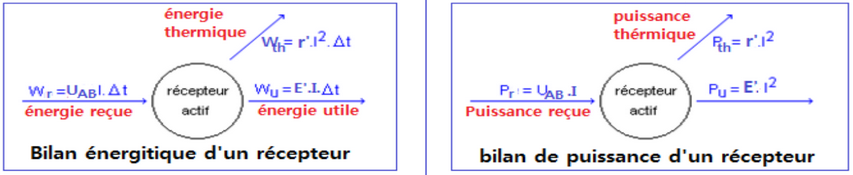
\includegraphics[width=0.7\textwidth]{./img/Puissance_utile_Pu_Pe.png}
\end{center}

\begin{wrapfigure}[10]{r}{0.3\textwidth}
    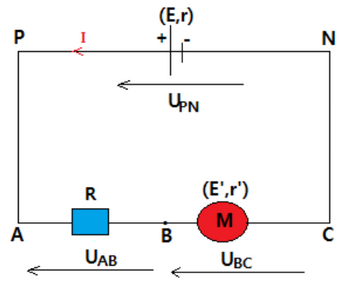
\includegraphics[width=0.3\textwidth]{./img/circuit_serie_morot_resistance.png}
\end{wrapfigure}


\section{Bilan énergétique d’un circuit simple : }
\subsection{Loi de Pouillet : }
On considère le circuit en série constitué par un
générateur, un moteur et un conducteur ohmique :
D’après la loi d’additivité des tensions et la loi
d’ohm on a :
$$U_{PN} = U_{AB} + U_{BC}$$
$$E - r. I = E' + r'.I + R. I$$
$$E - E' = (R + r + r').I$$
$$I = \frac{E-E'}{R + r +r'}$$
La généralisation de cette loi conduit à l’expression suivante :
$$I = \frac{\sum E - \sum E'}{\sum R}$$

\subsection{Bilan énergétique de circuit : }
On multipliant les deux membres de cette égalité par $I. \Delta{t}$ , on obtient :
$$(E - E').I.\Delta{t} = (R + r + r').I^2.\Delta{t}$$
$$E.I.\Delta{t} = E'.I.\Delta{t} + (R + r + r').I^2.\Delta{t}$$
$$W_g = W_u + W_{th}$$

$W_g = E.I.\Delta{t}$ : Energie totale fournie par le générateur.

$W_u = E'. I. \Delta{t}$ : Energie utile (mécanique pour le moteur).

$W_{th} = R.I^2.\Delta{t}$ : Energie thermique dissipée par effet joule.

\subsection{Rendement globale d’un circuit simple: }
Le rendement global de circuit est définit comme le rapport de l’énergie utile du circuit
par l’énergie totale ( du générateur).

$$\rho = \frac{W_u}{W_r} = \frac{P_u}{P_r} = \frac{E'.I.\Delta{t}}{E.I.\Delta{t}} = \frac{E'}{E}$$

\begin{wrapfigure}[10]{r}{0.4\textwidth}
  \vspace{-1cm}
    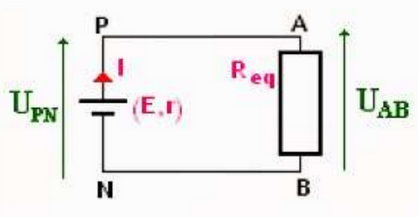
\includegraphics[width=0.4\textwidth]{./img/circuit_forceElectro.png}
\end{wrapfigure}


\section{Facteurs influençant sur l’énergie fournit par un générateur au reste d’un circuit résistif :}
\subsection{Influence de la force électromotrice : }
On considère le circuit suivant : 
$$U_{PN} = E - rI$$
$$U_{AB} = R_{eq}. I$$
Req : est la résistance équivalente du
dipôle AB.
D’après la loi de Pouillet on a : $I =\frac{E}{r + R_{eq}}$
L’énergie électrique fournie par un générateur pendant la durée $\Delta{t}$ est : $W_{ex} = U_{PN}.I. \Delta{t}$
$$W_{ex} = R_{eq}.I^2.\Delta{t} = \frac{R_{eq}}{(r + R_{eq})^2}.E^2.\Delta{t}$$
La puissance électrique fournie par un générateur est proportionnelle au carré de sa
force électromotrice.

\begin{wrapfigure}[10]{r}{0.4\textwidth}
    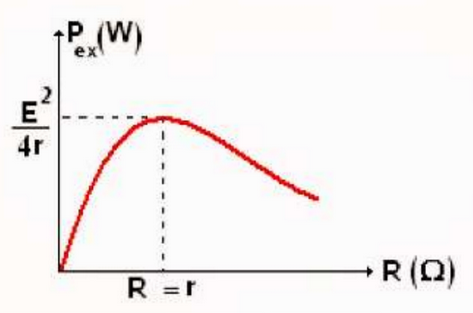
\includegraphics[width=0.4\textwidth]{./img/Influence _Resistance.png}
\end{wrapfigure}


\subsection{Influence des résistances et de leurs modes d’association : }

\subsubsection{Influence de la résistance : }
On considère le dipôle AB précédent est un conducteur ohmique de résistance R.
L’énergie électrique fournie par un
générateur pendant la durée $\Delta{t}$ est :
$$W_{ex} = U_{PN}. I. \Delta{t}$$
$$W_{ex} = R.I^2.\Delta{t} = \frac{R}{(r + R)^2} .E^2.\Delta{t}$$
En mathématique, pour une valeur donnée
de la force électromotrice, la puissance 

$Pe_{max}$ est maximale quand R = r. Son expression est :$Pe_{max} = \frac{E^2}{4.r}$

\subsubsection{Influence de mode d’association : }

\begin{center}
  \bf{Association en série }
\end{center}
\begin{wrapfigure}[10]{r}{0.2\textwidth}
  \vspace{-1cm}
    \includegraphics[width=0.2\textwidth]{./img/-Association en parallèle.png}
\end{wrapfigure}

La puissance électrique fournie par le générateur aux deux
conducteurs ohmiques est : $ P = U_{AB}.I = E. I$
$$I = \frac{E}{R_{eq}} et R_{eq} = R_1 + R_2$$
$$P = \frac{E^2}{R_1 + R_2}$$

\begin{center}
  \bf{Association en parallèle}
\end{center}
\begin{wrapfigure}[10]{r}{0.2\textwidth}
  \vspace{-4cm}
    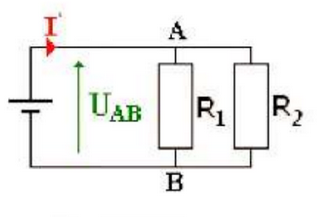
\includegraphics[width=0.2\textwidth]{./img/circxuit_parallele.png}
\end{wrapfigure}


La puissance électrique fournie par le générateur aux deux conducteurs ohmiques
est : $ P' = U_{AB}.I = E. I'$
$$I' = \frac{E}{R'_{eq}} et R_{eq} = R_1 // R_2 = \frac{R1.R2}{R1 + R2}$$
$$P = \frac{E^2}{R_1.R_2}.(R_1 + R_2)^2$$


Conclusion :
$\frac{P'}{P} = \frac{(R_1 + R_2)^2}{R_1.R_2} > 1 $ donc $P' > P$
La puissance électrique fournie par un générateur à des conducteurs ohmiques
montés en parallèle est supérieur à la puissance électrique fournie par ce générateur à
ces conducteurs ohmiques montés en série.

\section{limites de fonctionnement des générateurs et des récepteurs : }
\subsection{Générateurs : }
Une alimentation stabilisée de tension fournie une intensité de courant constante tant
que cette intensité ne dépasse pas une valeur limite indiquée par le constructeur :
$$Pmax = E. I_{max}$$
\subsection{Conducteurs ohmiques : }
Chaque conducteur ohmique est caractérisé par sa résistance R et sa puissance
maximale Pmax qu’il peut dissipée par effet Joule.
$$P_{max} = U_{max}.I_{max} = R.I^2_{max} = \frac{U_{max}^2}{R}$$

Exprimons Imax et Umax que le conducteur peut supporter :
$$I_{max} = \sqrt{\frac{P_{max}}{R}} et U_{max} = \sqrt{R.P_{max}}$$




\end{document}

